\documentclass[12pt]{article}
%compile using XeLaTeX
\usepackage{diary_style}
\setlength{\footskip}{\paperheight
  -(0.75in+\voffset+\topmargin+\headheight+\headsep+\textheight)
  -0.75in}

%\fontspec{Times New Roman}

\DeclareMathOperator{\di}{d\!}
\newcommand*\Eval[3]{\left.#1\right\rvert_{#2}^{#3}}

\begin{document}

%\doublespacing
\vspace{1.0 \baselineskip}

\begin{flushright}
	Alexander Caines\\
	MATH-310\\
	3-23-2021\\
\end{flushright}

\begin{center}
	\textbf{\underline{HMWK 3}}
	\emph{With help from Stephanie.}
\end{center}


%\vspace{0.5 \baselineskip}

\begin{enumerate}
	\item[(1)] Assume that the differences between the variances of the data are not statistically significant. A two-way
		 ANOV is necessary here because there are multiple independent factors being considered.\\
		\begin{enumerate}
			\item[(a)] Consider the following null hypotheses: That fiber, sand, or sandfiber have no statistically significant 
			effect on wetmold strength. The corresponding alternative hypotheses being that fiber, sand, or sand-fiber had 
			statistically significant effects on wetmold strength. The results of the ANOVA showed that, at the 95\% 
			significance level, the 
			only factor that contributed a statistically significant effect on wetmold strength was fiber. So, 
			we can reject the null that fiber had no effect on wetmold strength. Because sand and sand-fiber 
			did not have a statistically significant effect on wetmold strength, we fail to reject the null that 
			either of them did.\\ 
			\item[(b)] Consider the following null hypotheses: That fiber, sand, or sandfiber have no statistically significant 
			effect on casting hardness. The corresponding alternative hypotheses are that: fiber, sand, or sandfiber have a 
			statistically significant effect on casting hardness. The results of the ANOVA showed that fiber and sand have a 
			statistically significant effect on casting hardness at the 95\% confidence level. So, we can reject the null 
			hypothesis that either of the two do not. Since sand-fiber has a statistically significant effect on casting hardness, 
			however, we fail to reject the null that it doesn't. 
			\item[(c)] I tried to make a plot but it honestly didn't show any 
			of the results Stephanie and I got for a and b. So, I am confused.
		\end{enumerate}
	\item[(2)] Because none of the elements in the F-Stat column are less than 0.05, it can be conclulded that there 
	is no significance in effects between the fixed factors listed in the problem on the strength of paper. Find the ANOVA table below.\\
		\begin{center}
			\begin{tabular}{c|c|c|c|c}
				& SS & dof & msq & f-stat\\
				\hline
				A & 6.94 & 1 & 6.94 & 19.83\\
				B & 5.61 & 3 & 1.87 & 5.34\\
				C & 12.33 & 2 & 6.17 & 17.61\\
				AB & 14.40 & 3 & 4.8 & 13.71\\
				AC & 27.32 & 2 & 3.66 & 10.46\\
				BC & 15.80 & 6 & 2.63 & 7.52\\
				SSE & 8.42 & 24 & 0.35 & \\
				\hline
				SST & 70.82 & 32 & 2.21 & \\
			%	A & 6.94 & 1 & 6.94 & 2.97\\
			%	B & 3.61 & 3 & 1.20 & 0.51\\
			%	C & 12.33 & 2 & 6.17 & 0.38\\
			%	AB & 4.05 & 1 & 4.03 & 4.73\\
			%	Error & 14.04 & 6 & 2.34 & \\
			%	Total & 40.7 & 13 & 20.68 & \\
			\end{tabular}
		\end{center}
\newpage
	\item[(3)] The ANOVA showed that each of the factors did not exhibit a statistically significant effect on the life of a tool at the 
		95\% significance level. 
		\begin{figure}[!h]
			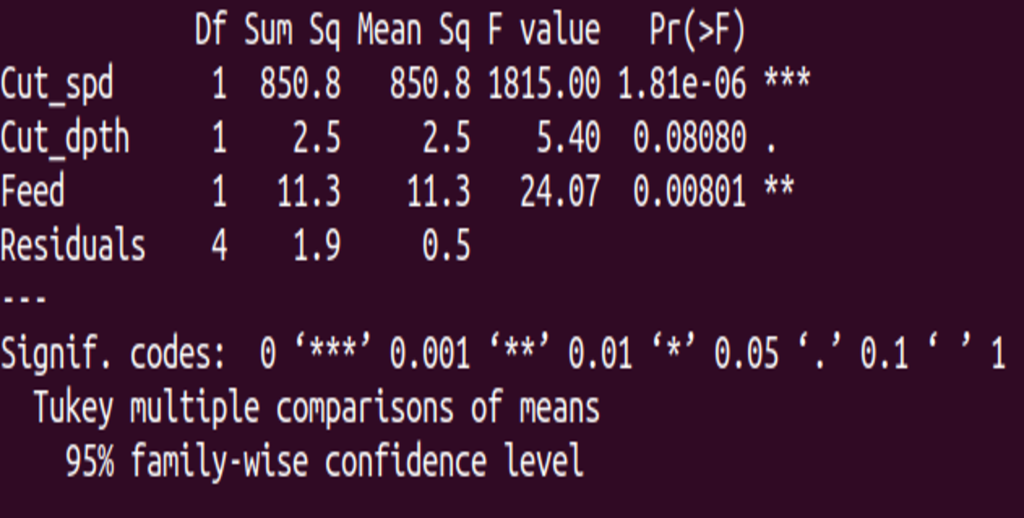
\includegraphics[width=\linewidth, height = 5cm]{anova3.png}
			\caption{ANOVA results}
		\end{figure}
	\item[(4)] Given $y = 4000 + 10x$, we know that $Y = 6000 + \epsilon$, where $\epsilon = 500$. The reason it can't be the case that both probablities can't hold is because 
	the epsilon must be constant between the two as the variance is constant between 
	elements in the dataset.\footnote{I don't think this response makes any sense.}
	\item[(5)]  Consider the following deductions.
		\begin{center}
			\begin{math}
				\begin{aligned}
					nb_0 + (\sum x_i)b_1 &= n(\frac{\sum y_i - \beta^{hat}\sum x_i}{n}) + \sum x_i \cdot \bigg(\frac{\sum (x_i - \bar{x})(y_i - \bar{y})}{\sum(x_i - \bar{x})^2} \bigg)\\
					&= \sum y_i + \sum x_i \cdot \bigg(\frac{\sum (x_i - \bar{x})(y_i - \bar{y})}{\sum(x_i - \bar{x})^2} - \hat{\beta_1} \bigg)\\
					&= \sum y_i + \sum x_i (\hat{\beta_1} - \hat{\beta_1})\\
					&= \sum y_i
				\end{aligned}
			\end{math}
		\end{center}

		\begin{center}
			\begin{math}
				\begin{aligned}
					I didn't get around to proving this.
				\end{aligned}
			\end{math}
		\end{center}
	\item[(6)] Let $\bar{x}$ and $\bar{y}$ be the respective means of points $(x,y)$ modeled by a linear regression of the form $Y = \beta_0 + \beta_1 x + \epsilon$. Note, that 
		for $n$ samples, $\bar{x} = \frac{1}{n}\sum (\hat{x_i} + \epsilon_i)$ 
and $\bar{y} = \frac{1}{n}\sum (\hat{y_i} + \epsilon_i)$. Note, that the epsilons 
		eventually sum to zero\footnote{Somehow. This has to work for the approximation to equal the true mean}. So, $\bar{x} = \hat{x}$ and $\bar{y} = \hat{y}$. So, 
		the approximation given by the regression $(\hat{x}, \hat{y})$ passes 
		through the point average $(\bar{x}, \bar{y})$.
\end{enumerate}

\end{document}
